\section{Component Overview}\label{sec:componentOverview}
Figure \ref{fig:sysArch} contains the high-level overview of the system that
we will use for query evaluation. We will now give a brief explanation of the
components present in this figure:
\begin{enumerate}
    \item \textbf{LDBC}: The Linked Data Benchmark Council(LDBC) publishes datasets
        for various types of graph processing workloads. In this thesis, we make
        use of the Social Network Benchmark (SNB) datasets in order to evaluate
        the performance of our traversals.
    \item \textbf{LDBC Converter}: The LDBC dataset are in CSV format and
        contain additional information about nodes and edges. As we will explain
        in Section \ref{sec:modifiedCsr}, we need the data to be in a particular
        binary format and we do not have any use for node and edge properties.
        This component of the system removes the unnecessary information from
        the LDBC datasets and maps the data into the desired binary format.
    \item \textbf{AWS S3}: Once the LDBC converter converts the data into a
        binary format, this data is added to an AWS S3 bucket. A `bucket' in AWS S3
        is a container for files.
    \item \textbf{Graph Access Service}: This service provides an interface for
        accessing a graph stored in AWS S3. This interface provides its users
        the ability to get a node's neighbours by providing
        the source node, edge label, and edge direction. This service contains
        all the caching mechanisms that we will use to reduce the latency of
        traversals. We will discuss this service in more detail in
        Section \ref{sec:graphAccess}.
    \item \textbf{Graph Algorithm Service}: This service is responsible for
        using the interface provided by the graph access service to perform
        traversals and measure their performance. We discuss this component in
        more detail in Section \ref{sec:parallelAlgorithms}.
\end{enumerate}
\begin{figure}[ht]
    \centering
    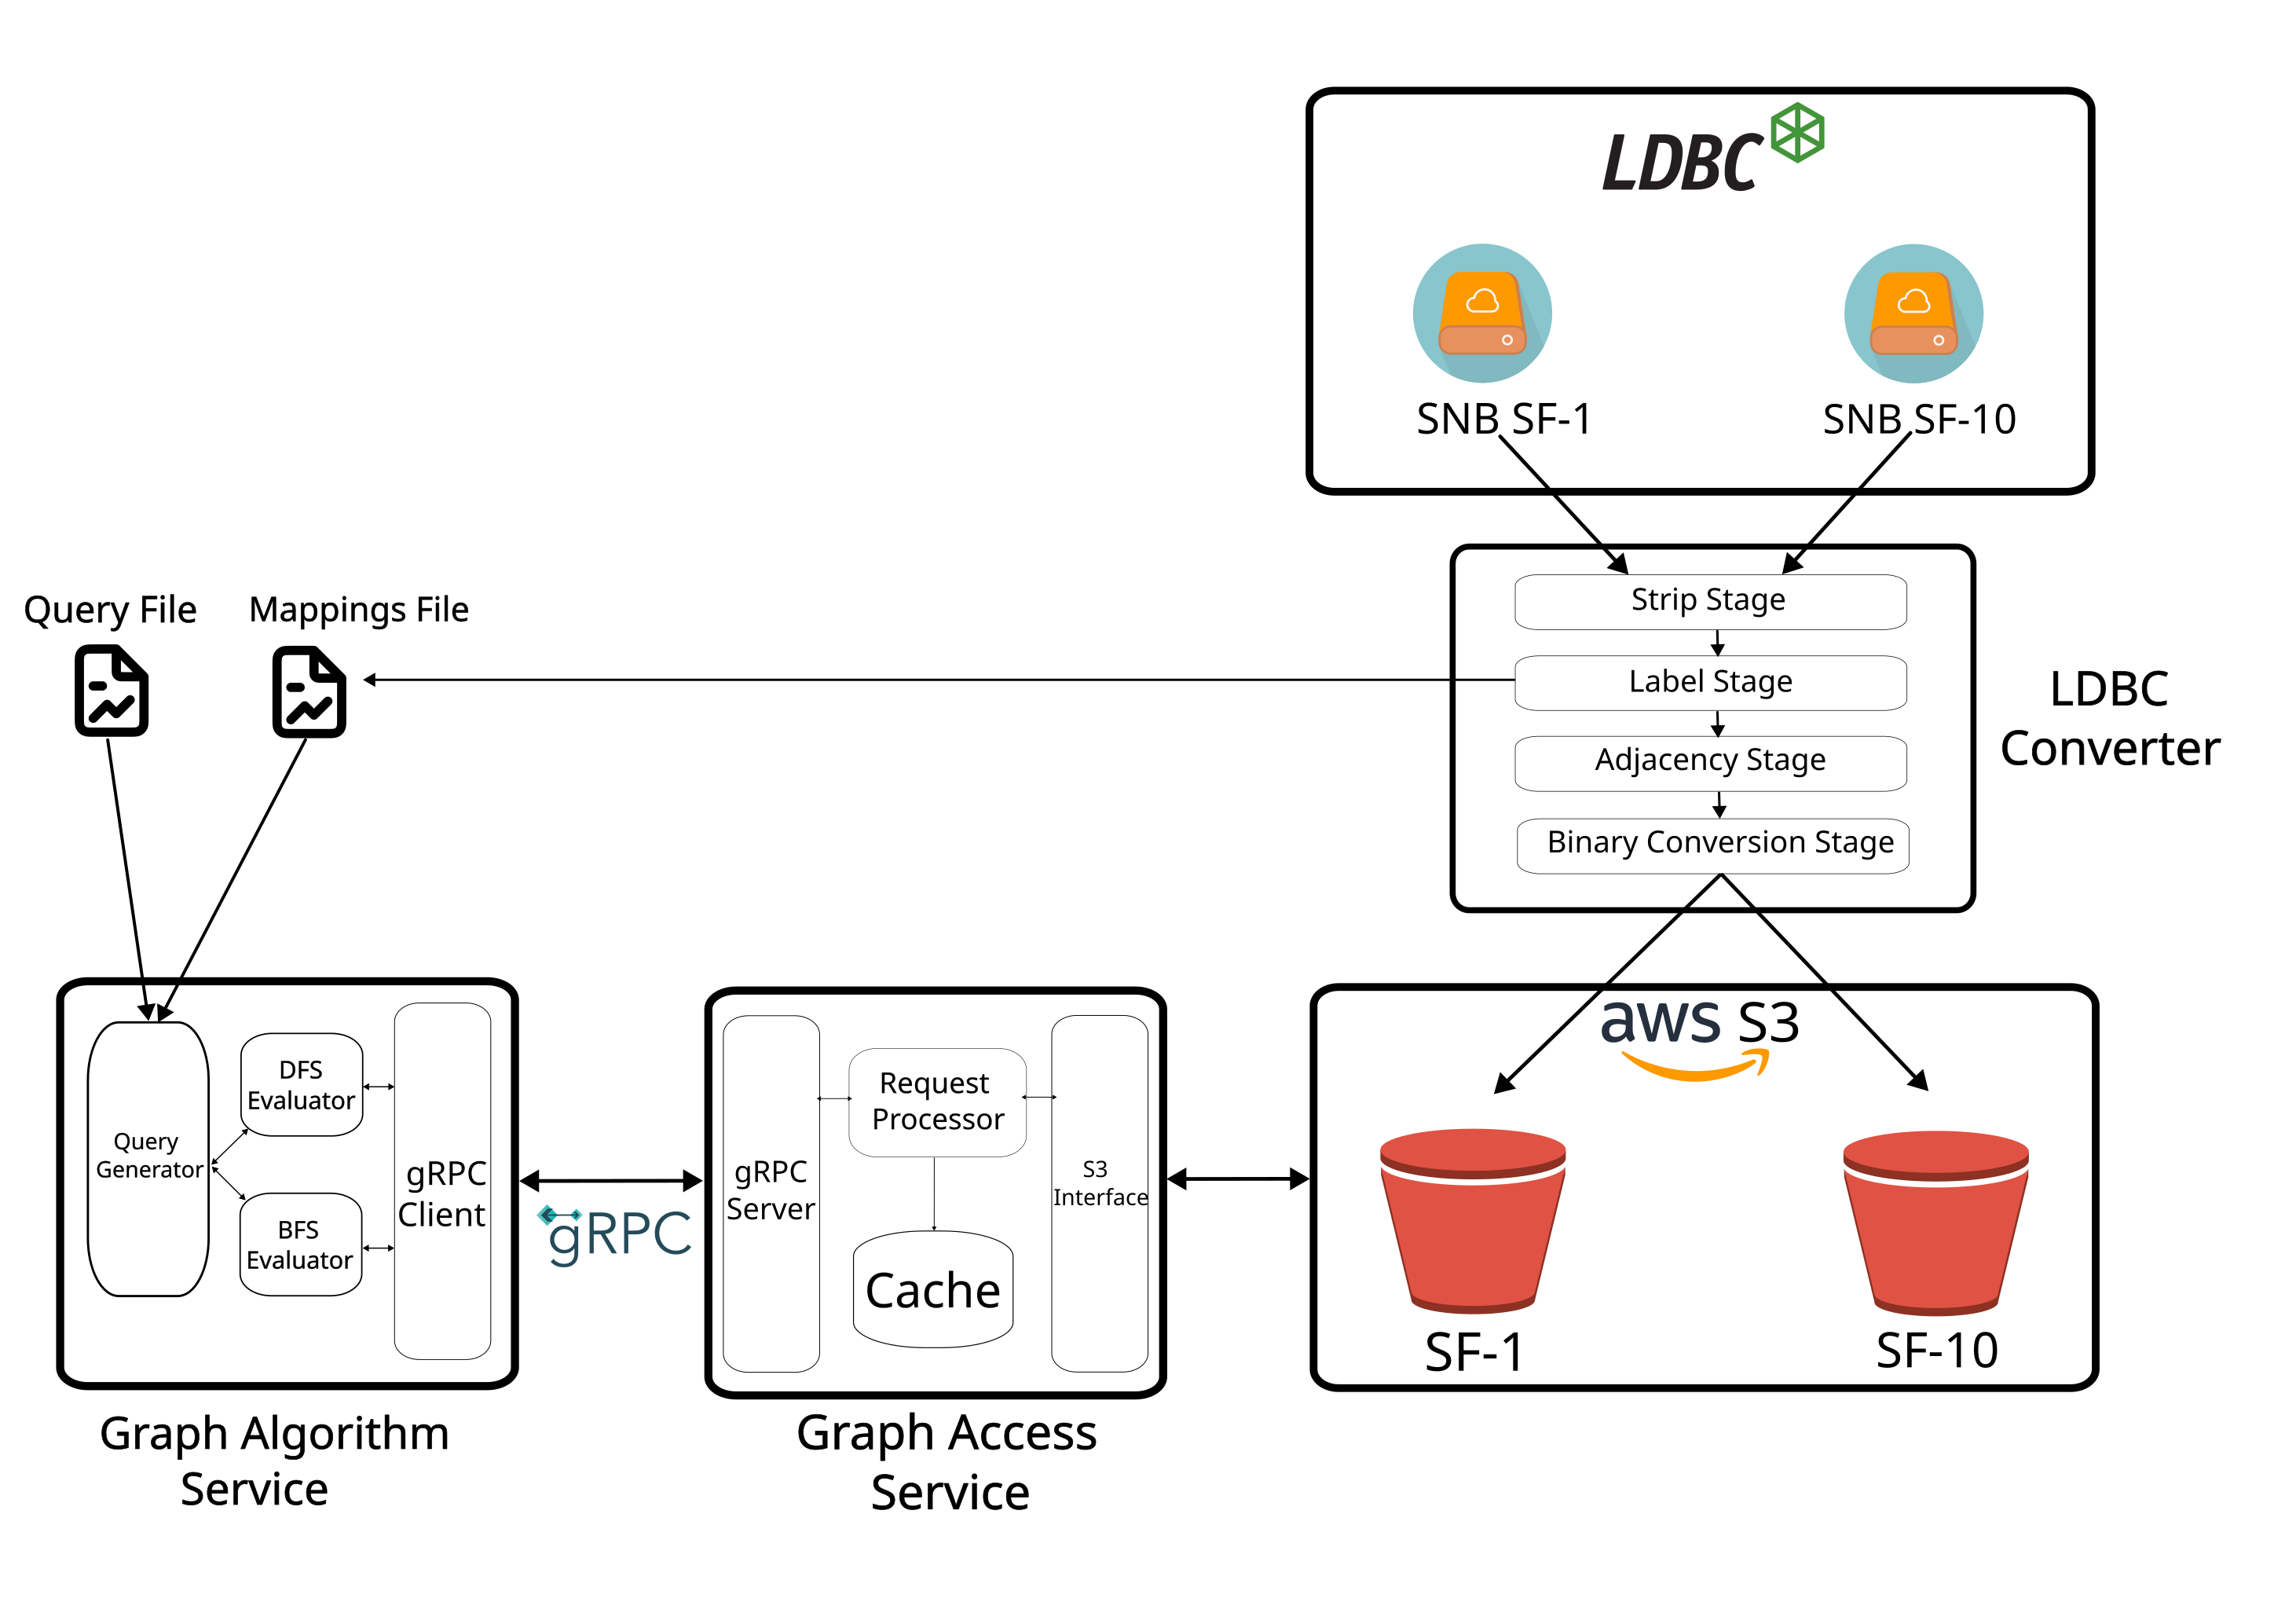
\includegraphics[width=0.9\textwidth]{figures/architecture.png}
    \caption{High Level System Architecture}
    \label{fig:sysArch}
\end{figure}

Looking at the architecture in Figure \ref{fig:sysArch}, it is natural to wonder
why we have two separate services for accessing the graph and performing
traversals on that graph. There are two reasons for this separation: first, it
separates the logic for accessing graphs from the logic for performing
traversals with minimal overhead; second, this type of architecture is
particularly amenable to creation of a multi-tenant storage layer, as used
in the Neon database \cite{neonPostgres}. This is why we have chosen to separate
the service responsible for accessing the graph and caching from the service
responsible for running traversal algorithms.

\section{Baseline Implementation}\label{sec:baseline}
Since there are no existing tools that we can use to compare our solution with,
we present a baseline implementation to gauge the effectiveness of our caching
techniques and algorithmic improvements that we will present in the following
sections. The main idea of the baseline implementation is to provide the most
straightforward way to perform traversals on a graph that is stored in AWS S3.

\medskip
As per the workflow we presented in Section \ref{sec:componentOverview}, we
first need to convert the graph from the LDBC dataset into a format that
enables us to fetch parts of the graph that we need for processing. In order to
do this, we convert the graph into an adjacency list, then we partition that
adjacency list based on size, and finally convert it to compressed sparse
row (CSR) format \cite{duff1984computer}. With this partitioned CSR format stored
in AWS S3, our aim is to load the desired file whenever we want to fetch a node's
neighbours.

\medskip
Figure \ref{fig:baselineImpl} shows the design of graph access service and graph
algorithm service for this baseline implementation. The graph algorithm service,
is responsible for performing the traversals and recording the results. This
service uses the textbook implementation of DFS and BFS, with the only caveat
that a node's neighbours are requested from the graph access service. The graph
access service contains an index which maps node ranges to AWS S3's file names. With
this index, we can get the file name for the AWS S3 file which contains a particular
node's neighbours. Additionally, this service also contains an LRU cache of some
files that were fetched from AWS S3. The size of this cache is limited because each
cache entry contains an entire file with adjacency information for
hundreds of nodes. With these components in place, whenever the graph access
service gets a request, it first checks if that request can be served from the
cache; if not, we fetch the file corresponding to the requested node and add
that file to the cache.
\begin{figure}[ht]
    \centering
    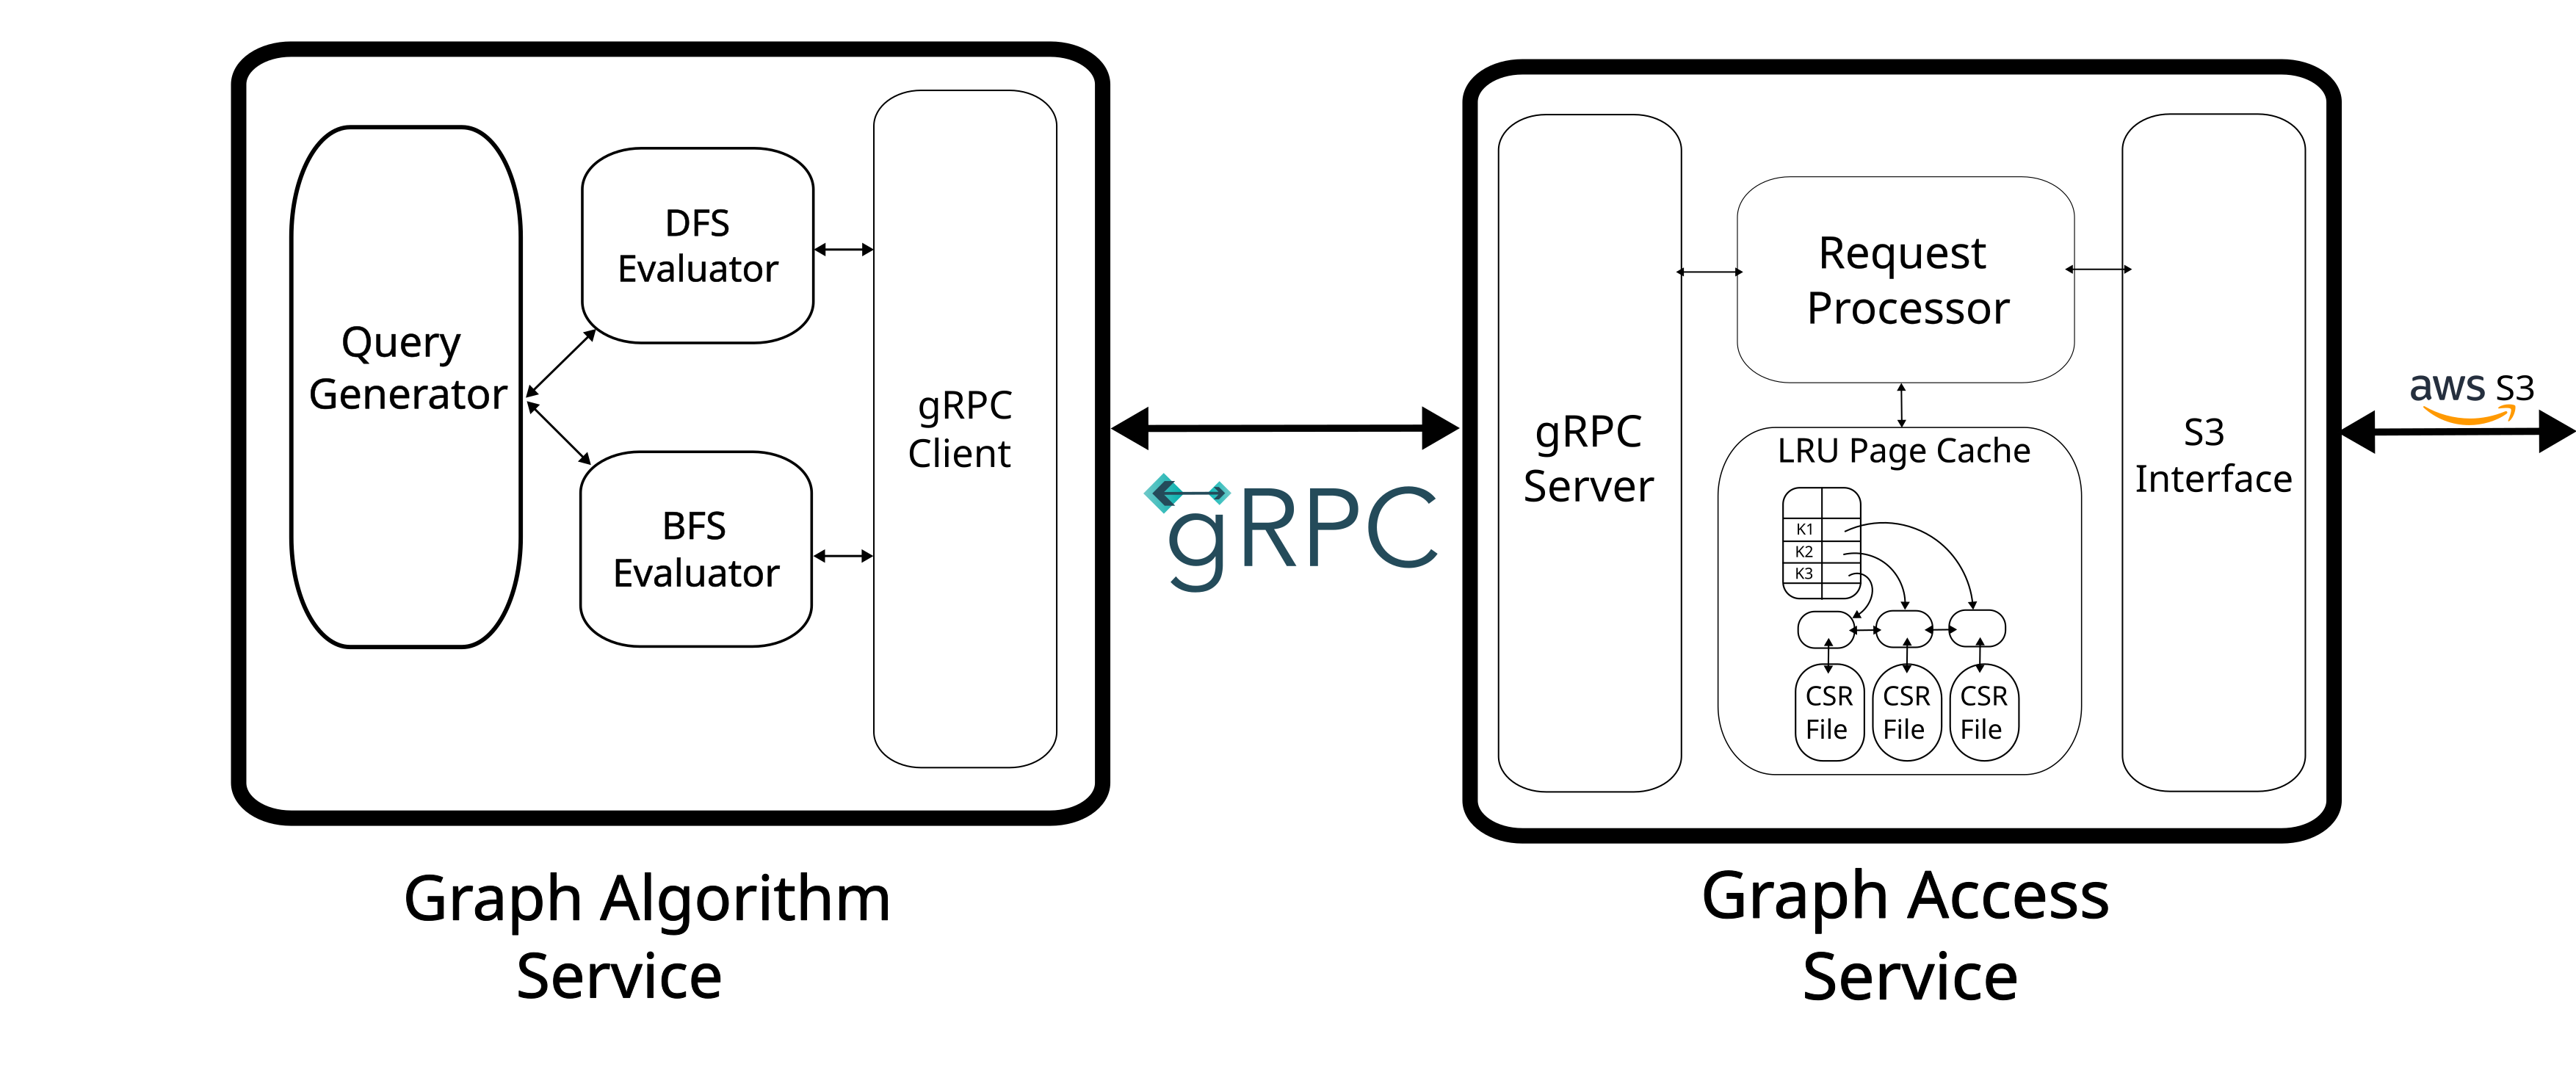
\includegraphics[width=0.8\textwidth]{figures/baseline.png}
    \caption{Baseline Implementation}
    \label{fig:baselineImpl}
\end{figure}

\medskip
The approach described in this section is quite straightforward but there are
various improvements that can be done to improve the performance and to better 
leverage the features provided by AWS S3. In the next few sections, we will
discuss how we can improve the implementation for both the graph access service
as well as the graph algorithm service. 

\section{Graph access service}\label{sec:graphAccess}
In this section, we first describe a modification of the CSR format in
Section \ref{sec:modifiedCsr} which will help us improve our cache performance.
In Section \ref{sec:accessCachePrefetching}, we describe how we leverage
this updated file format and employ the caching schemes mentioned in
Section \ref{sec:cachingDistSys}.

\subsection{Modified CSR structure}\label{sec:modifiedCsr}
In the baseline implementation of graph access service described in
Section \ref{sec:baseline}, we had to download entire files to access
a node's neighbours. This approach suffers from a couple of problems, which makes
fetching inefficient and restrictive. The first problem is that we have to
fetch and parse the information for an entire file in order to access a single
node's neighbours which is wasteful. Furthermore, this approach hinders our
ability to achieve a  higher level of granularity for better cache performance.
Second, this approach makes it harder to utilize the fact that AWS S3 replicates
files to various servers. Due to these problems, we decided to modify the
underlying binary format and the way we fetch a node's neighbours.

\medskip
Figure \ref{fig:csrFormat} shows the binary format we use for fetching a
node's neighbour. This format can logically be divided into three layers. The
first layer, which is always of a constant size, contains the first and last
node identifier present in this file. The second layer contains the byte offset
for the first incoming edge for a node and the first outgoing edge for a node.
Since these offsets are of a constant size and the fact that the first layer of
the header indicates how many nodes are present in this file, we can calculate
the size of this second layer. The third and final layer contains the edge
information, which in our case consists of the edge label and the edge
destination. This type of structure closely resembles a traditional CSR format
except for the fact that we store both incoming and outgoing edges in the same
array and that we store byte offsets instead of array indices.
\begin{figure}[ht]
    \centering
    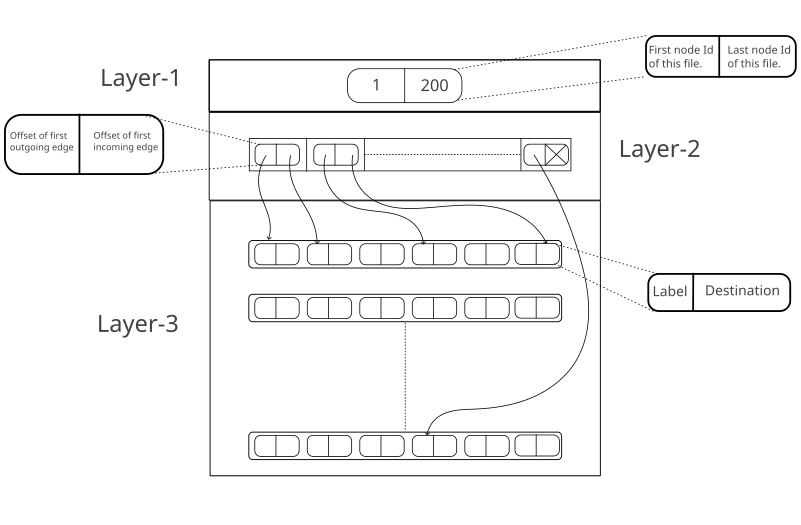
\includegraphics[width=0.8\textwidth]{figures/csrFormat.png}
    \caption{Updated CSR Format}
    \label{fig:csrFormat}
\end{figure}

\medskip
The aforementioned format gives us the ability to fetch a node's neighbours
without having to download an entire file. With this modified structure, we can
store the first layer of every file in memory and fetch the second layer of a
file when it is first accessed. After doing so, we would be able to fetch a
node's incoming or outgoing neighbours without any additional overhead.
Furthermore, we can now parallelize requests to a single file, which would lead
to better throughput since these requests would likely be distributed to
different instances within AWS S3. As an additional benefit, we can now perform
caching on a more granular level since we do not incur the overhead of fetching
and parsing an entire file whenever we need to access a node's neighbours.

\subsection{Caching and Prefetching}\label{sec:accessCachePrefetching}
Figure \ref{fig:graphAccessArch} shows the final architecture of the graph
access service. The service consists of three basic parts:
\begin{enumerate}
    \item \textbf{Interfaces for external communication}: There are two 
        components which provide an interface with external resources and are
        colored grey in the figure. The first component, on the left,
        exposes a gRPC interface which receives requests for accessing a node's
        neighbours, starting traversals, and ending traversals. The second
        component, on the right, is responsible for accessing AWS S3. This component
        takes a filename along with starting and ending file offsets and returns
        the requested file content.
    \item \textbf{Orchestration}: There are two components that help with
        orchestration of request and are colored blue in the figure. The first
        component is the `Request Processor' which is responsible for
        interacting with the caches, moving data between caches, and fetching
        data from AWS S3 in case it is not present in the caches. The second
        component titled `Vertex offsets' contains metadata related to the CSR
        format that we described in Section \ref{sec:modifiedCsr}.
    \item \textbf{Caches}: There are two different types of caches that are used
        in this service and are colored green in the figure. The first of these
        components is an LRFU cache which is used to store nodes that were
        previously accessed. The second component is a per-query prefetcher
        which fetches the nodes that are likely to be accessed by a client in
        the near future. The rest of this section is devoted to the description
        of these two components.
\end{enumerate}
\begin{figure}[ht]
    \centering
    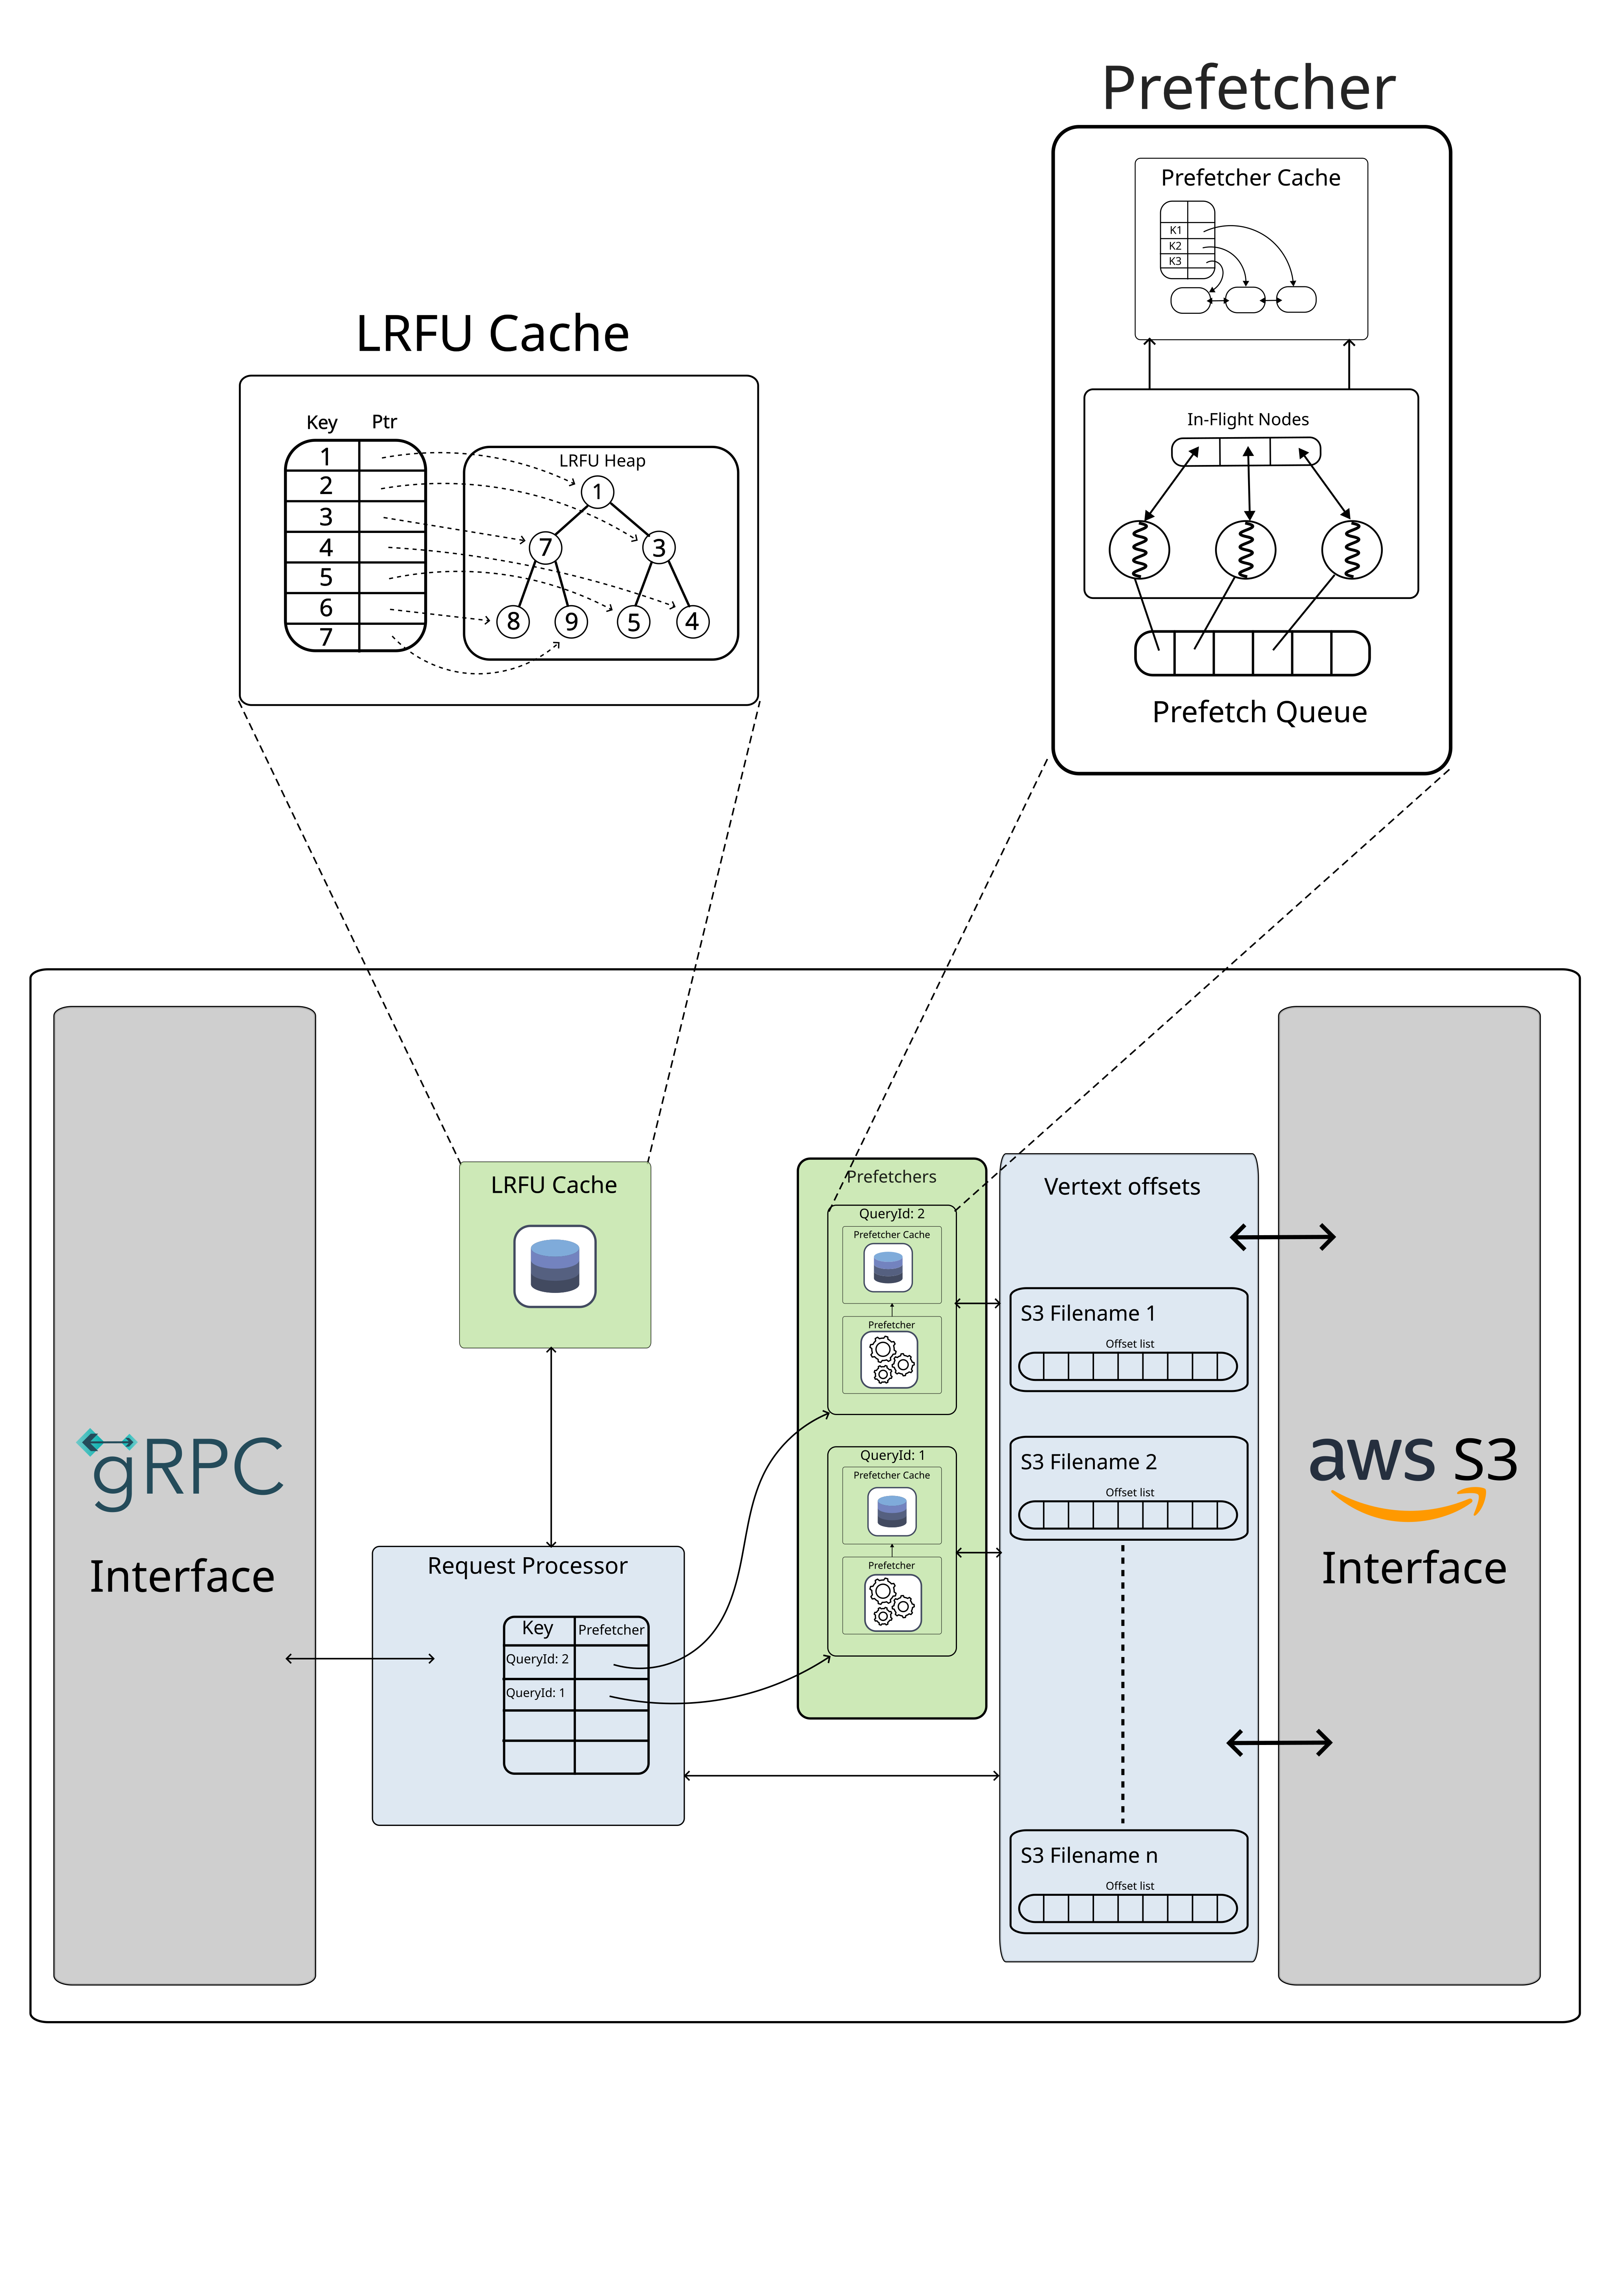
\includegraphics[width=\textwidth]{figures/graphAccessServiceFinal.png}
    \caption{Graph Access Service}
    \label{fig:graphAccessArch}
\end{figure}

\medskip
The first major component of our cache in the \textbf{LRFU
cache}\cite{lee2001lrfu}. As mentioned in Section \ref{sec:cachingDistSys}, the
main idea of this cache is to take both recency and frequency into account while
making the decision about which item to evict from the cache. While initializing
this cache, we make a decision about how much weight should be given to an
objects recency versus its frequency. Note that unlike perfect-LFU schemes, we
only store the frequency of the elements present in the cache. After
initializing the cache, it maintains a heap of elements where each element is
assigned a score based on the last time it was accessed along with its
frequency. The key to maintaining this heap is the realization that the relative
ordering of the heap remains constant if none of the elements are accessed. This
is because the degradation of score due to ageing happens at the same
rate for every element. This means that only a change in frequency can alter
the relative ordering of elements, and since the frequency only changes when an
object is accessed, we only need to change the position of the accessed node
within the heap. This enables us to perform access and insertion operations in
$\mathcal{O}(\log(n))$ time. Although simple LRU cache implementations have an
access and insertion time complexity of $\mathcal{O}(1)$,  this cache provides 
us with a good tradeoff between time complexity and flexibility for 
different workloads. We will talk more about the empirical evidence supporting
our choice in the next chapter.

\medskip
The next component, \textbf{the Prefetcher}, is inspired by the work done
by Bok et al. \cite{bok2020memory}. This component fetches the neighbours of
nodes that were accessed by a particular traversal. Every time a node's
neighbours are fetched, these neighbours are added to the `Prefetch Queue'. The
elements from this prefetch queue are read by the worker threads that are
attached to every prefetcher cache. These worker threads send our requests to
fetch the neighbours of nodes in the prefetch queue and add the nodes to the
`In-flight queue' while they wait for the response. Finally, once the neighbours
for a node are available, they are added to the prefetcher cache which is a
standard LRU cache. We will now discuss some of the design choices that we have
made for this cache.

\medskip
First, if there are multiple traversals happening, we would create a separate
prefetcher for each traversal. This choice ensures that there is minimal
interference on the performance of a traversal depending on other traversals
that may be happening. This comes with the added cost of having more worker
threads. However, using a green-thread model or asynchronous programming can help
mitigate this issue to a large extent. 

\medskip
Apart from separate prefetcher caches, we also have an `In-flight Queue' within
each prefetcher. This is useful because of the time gap between sending a
request and getting a response. This time, as we will see in the next chapter,
is an order of magnitude greater than the time scale at which the graph access
service and the graph algorithm service work. Therefore, it makes sense to have
a small amount of extra memory to ensure that if a request is already in
progress, we do not make a duplicate request, which would almost always take
longer to execute. 

\medskip
Finally, we note that the size of the prefetch queue is finite. Therefore, we
need to have some strategy to handle the case when this prefetch queue is full.
We argue that this strategy needs to be different for both BFS and DFS. This is
due to the relevance of nodes that are added to this prefetch queue. The node at
the front of the queue in BFS will be accessed earlier than the neighbours of a
node we are trying to add to the queue. However, in case of DFS, the
opposite is true because the node we are trying to add is likely the node
at the top of the stack and would be accessed next. This leads us to having two
different strategies for dealing with a full prefetcher queue for BFS and DFS:
\begin{enumerate}
    \item \textbf{BFS}: In case of BFS, the prefetcher queue behaves like a
        queue data structure and if the queue is full, the newer elements are
        discarded.
    \item \textbf{DFS}: In case of DFS, the prefetcher queue behaves like a
        stack data structure and if the queue is full, the newer elements
        are added to the top of the stack, and the elements at the bottom of the
        stack are discarded.
\end{enumerate}

\bigskip
In this section, we described a file format that enables us to perform caching
at a more granular level, and we described how this granular caching helps us
design caches that may be better suited for masking AWS S3's access latency.
In the next section, we turn our
attention to graph algorithm service where we will modify our traversals to
better fit the capabilities of AWS S3.


\section{Prallelizing traversals}\label{sec:parallelAlgorithms}
One of the main advantages of using AWS S3 is that it is able to sustain a very
high-throughput. The caching mechanisms mentioned in the previous sections
reduce the latency for accessing a node's neighbours and mitigate expensive
network calls to AWS S3 in the hot-path. These components do help with reducing
latency but they do not do anything to ensure that make use of the
high-throughput provided by AWS S3. In order to do that, we parallelize our
traversal algorithms. In this section, we will present parallel implementations
of BFS and DFS that would help us speed up our traversals by utilizing the
high-throughput of AWS S3.

\subsection{Parallel BFS}
Parallelizing breadth-first search in relatively straightforward.
Listing-\ref{lst:parallelBFS} contains the pseudo-code for our implementation of
parallel BFS. This implementation contains two queues, one for the current level
and the other for the next level of the traversal. Instead of processing the
current level within a single thread, we launch a predefined number of workers
who take elements from the queue at the current level in a work stealing
fashion and add their results to the next level of the traversal. The addition
of nodes to the next level as well as to the set of seen nodes needs to be
synchronized in accordance with the threading model of the language of
implementation.
\begin{lstlisting}[caption={Parallel BFS}, label={lst:parallelBFS}, captionpos=b, language=Python]
def ParallelBFS(startNode: nodeId, edgesToFollow: list[Edge]) -> list[nodeId] {
    startQueue = Queue[nodeId](startNode)
    for edge in edgesToFollow {
        nextLevelQueue = Queue[nodeId]()
        seen = Set[nodeId]()
        for i = 0; i < MAX_WORKERS; i++ {
            ## Use language provided utility to launch BFSWorker.
            launch_worker(startQueue, nextLevelQueue, seen, edge)
        }
        await_completion()

        startQueue = nextLevelQueue
    }

    return startQueue
}

## Operations on input, output, and seen are synchronized between
## workers. 
def BFSWorker(input, output: Queue[nodeId], seen: Set[nodeId], edge: Edge) {
    while (input.hasMoreElements()) {
        toProcess = input.Poll()
        neighbours = fetchNeighbours(toProcess, edge)
        for neighbour in neighbours {
            if neighbour not in seen {
                seen.add(neighbour)
                output.add(neighbour)
            }
        }
    }
}
\end{lstlisting}
Figure \ref{fig:parallelBFS} contains an example of how this algorithm would
work for a simple tree like graph shown on the left side of the figure. The
figure also contains three workers that are colored green, blue, and red.
This figure shows three iterations of the algorithm, along with how the
distribution of work might take place. We now describe each of these three
iterations:
\begin{enumerate}
    \item \textbf{Iteration 1}: In the first iteration, where we only have a
        single node, this node gets assigned to one of the workers at
        random. In this case it gets assigned to the green worker. At this
        stage, the green worker fetches the neighbours of this node and adds
        them to a shared set, which will be used as the starting point for the
        next iteration. In this case, the worker adds nodes 2,3,4, and 5 to this
        shared set.
    \item \textbf{Iteration 2}: In this iteration, the nodes from the shared set
        of the previous iteration are distributed among all three workers. Just
        like the previous iteration, every worker fetches the neighbours of the
        nodes assigned to them and adds the result to a shared set. In this
        iteration, nodes 2 and 3, which are assigned to different workers, try
        to add the node 7. This is the reason why we need a shared set,
        otherwise, we may end up processing node 7 twice in the next iteration.
    \item \textbf{Iteration 3}: Just like the previous iteration, the nodes from
        the shared set are distributed across workers. Subsequently, these
        workers add the neighbouring nodes of their assigned nodes to the shared
        set.
\end{enumerate}
\begin{figure}[ht]
    \centering
    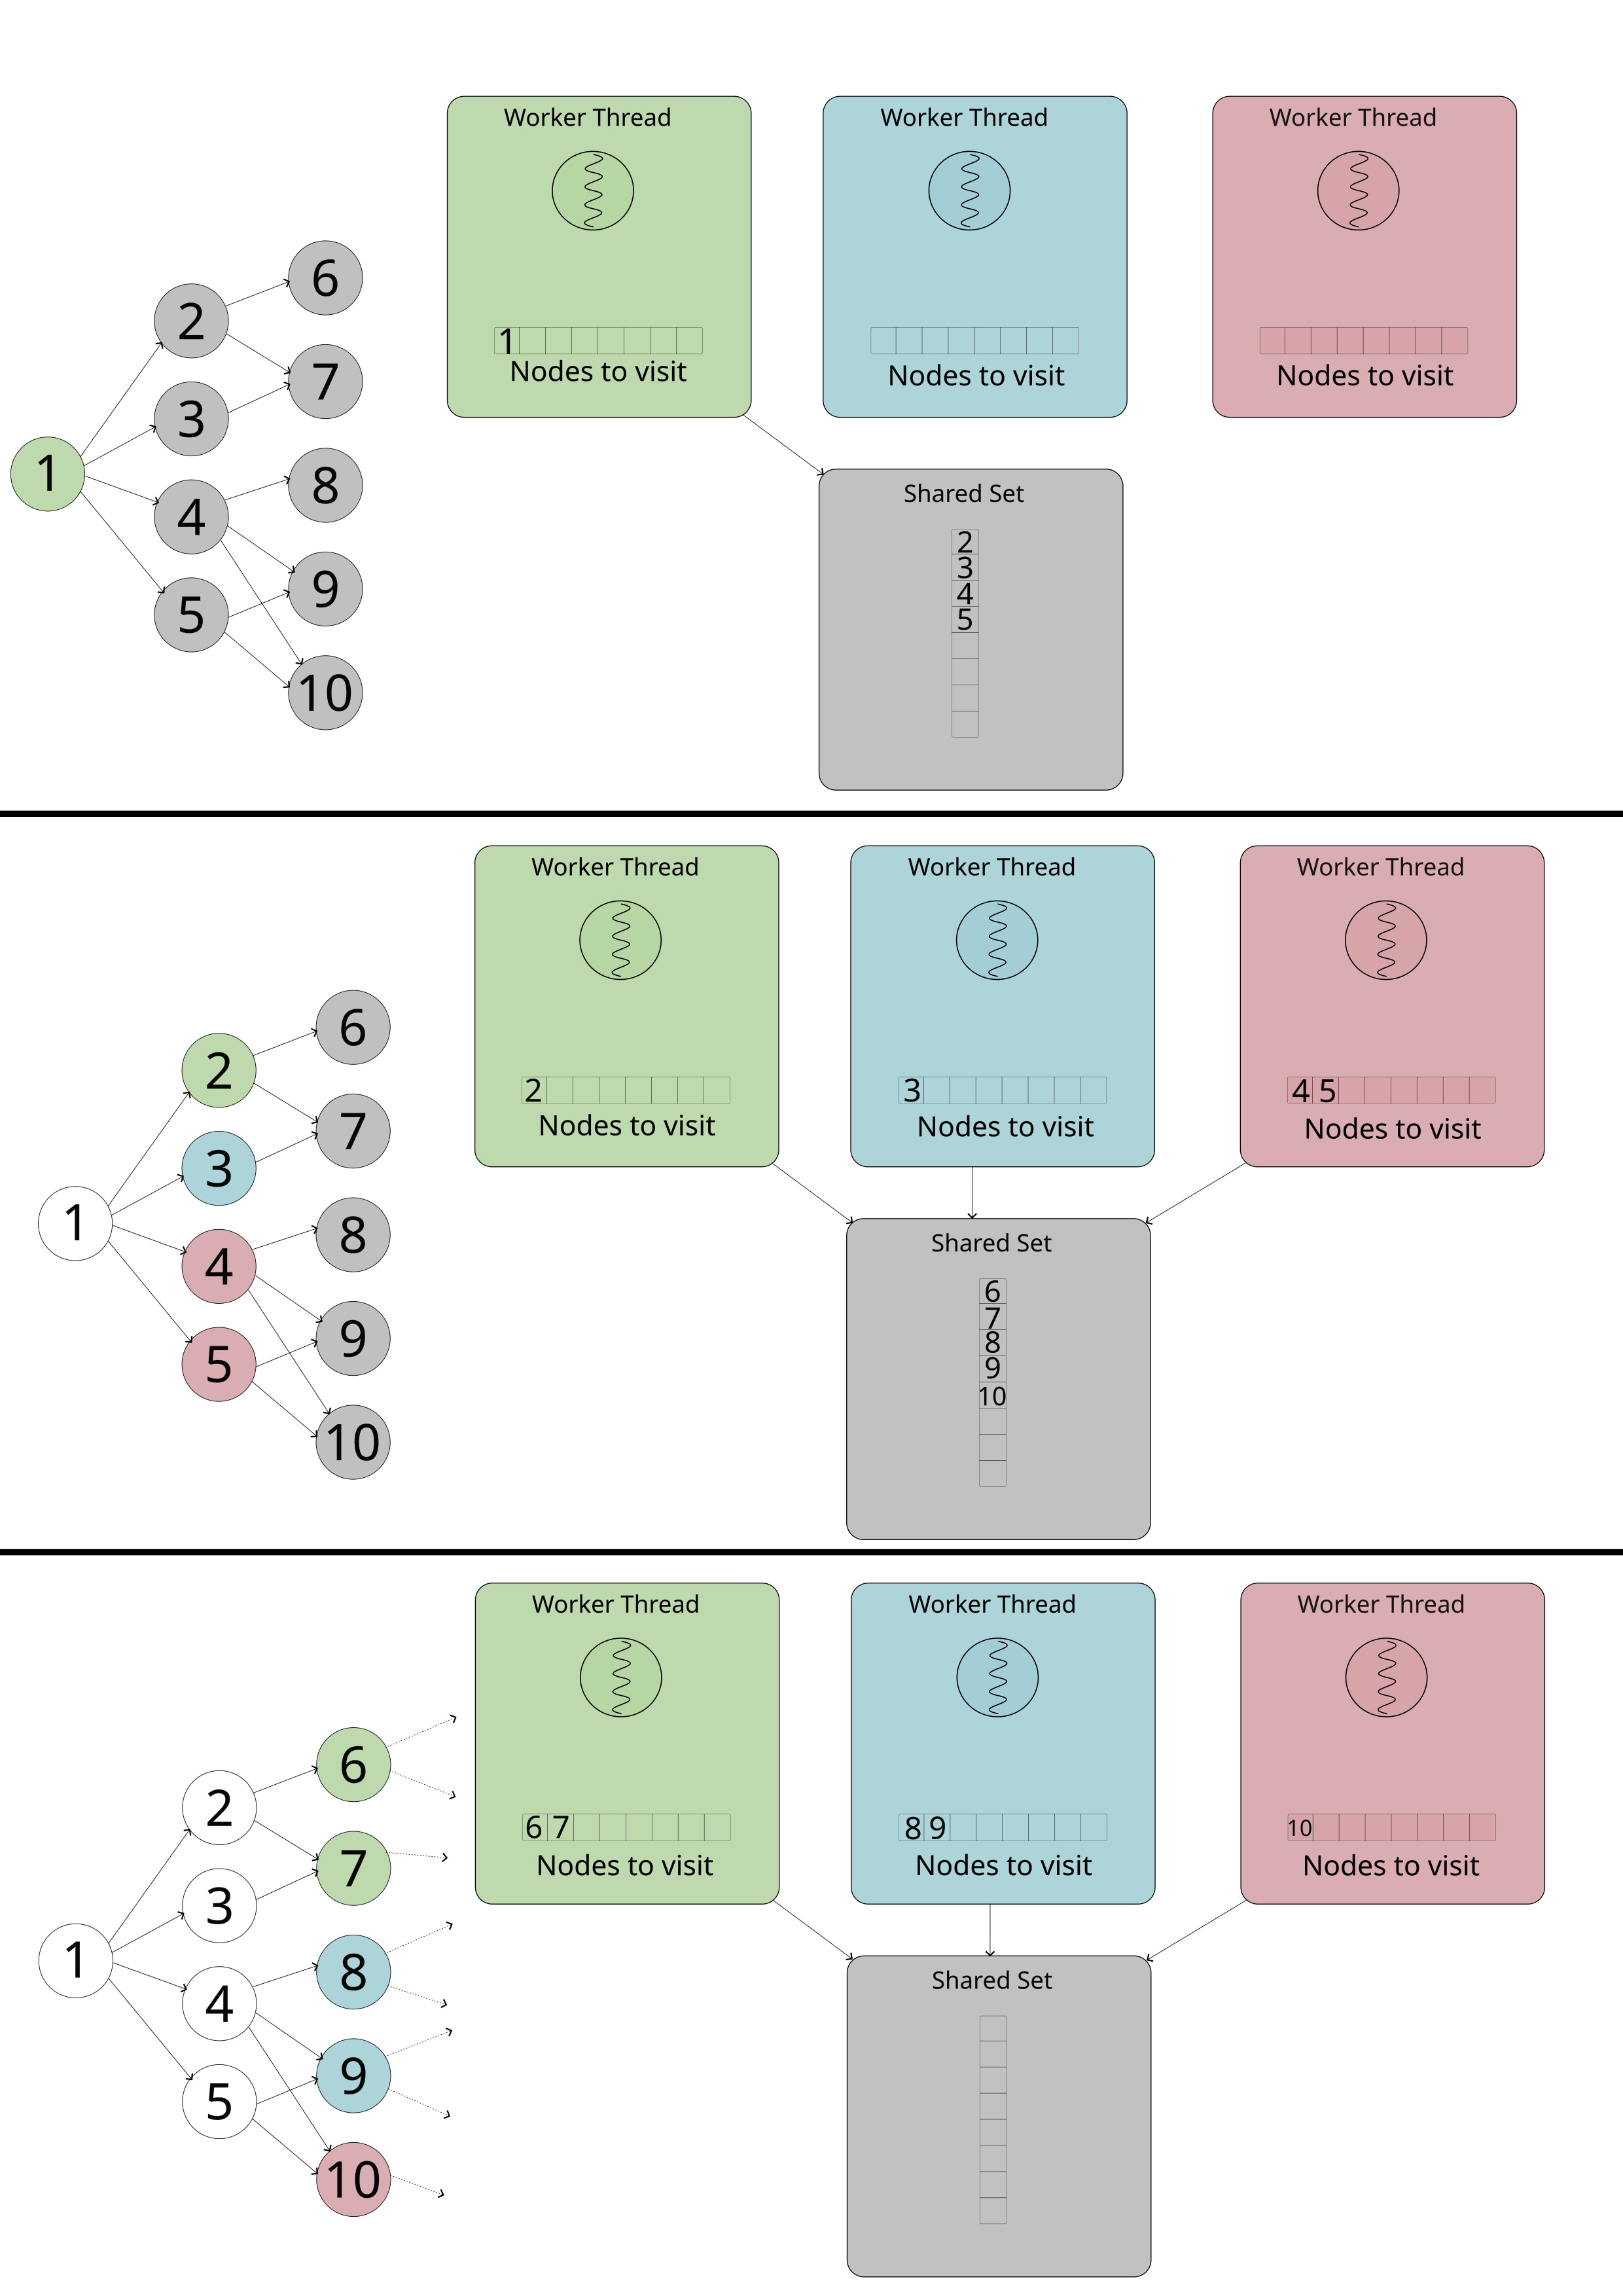
\includegraphics[width=0.75\textwidth]{figures/parallelBFS.png}
    \caption{Parallel BFS}
    \label{fig:parallelBFS}
\end{figure}

\subsection{Parallel DFS}
In this section, we describe our approach for parallelizing depth-first search.
Before we begin our description, it is important to note why a strategy similar
to the one described in the previous section would not result in equal
allocation of work. If we simply delegate the task on performing DFS on a node's
neighbours to different worker threads, then it is possible that some worker
threads might terminate significantly earlier than others. This is because the
number of nodes that can be explored from a given node might vary significantly
from one node to the other. Let us take the example of traversing a social
network graph where we start with a single person and find people connected to
this person till a certain depth. If the starting person has two friends `A' and
`B', let us assume that `A' has no friends while `B' is a celebrity and has many
friends. In this case, if we assign the work of perfroming DFS from `A' to one
worker and the work of performing DFS from `B' to another worker, we would end
up with an uneven distribution of work. This is because performing DFS on `A'
would require no further processing while the DFS on `B' is likely to go on for
quite a few iterations. Due to this problem, we need a better way to parallelize
depth-first search.

\medskip
The main idea of our approach is to dynamically rebalance the amount of work
being done by each worker in every iteration. One way to perform this dynamic
rebalancing was suggested by Rao et al.\cite{rao1987parallel} where they suggest
a work stealing algorithm in which a worker `steals' nodes from other workers'
stacks when its own stack becomes empty. Our algorithm, as shown in 
Listing-\ref{lst:parallelDFS} works on a similar principle. The one notable
difference is that instead of stealing work, every worker proactively assigns
work to different workers after fetching a node's neighbours which ensures that
the difference between the amount of work is minimized. Another important point
to note about the implementation is the structure of the data structure that
stores seen nodes. Instead of simply storing nodeIds, we store nodeId along with
the level at which a node was seen. This is done to ensure that for a traversal
with max depth `d', we return all the nodes that can be reached by taking `d'
steps from the source node.
\begin{lstlisting}[caption={Parallel DFS}, label={lst:parallelDFS}, captionpos=b, language=Python]
def ParallelDFS(startNode: nodeId, edgesToFollow: list[Edge]) -> list[nodeId] {
    stack = Stack[nodeId, level]((startNode, 0))
    seen = Set[nodeId, level]()
    result = Collection[nodeId]

    while stack.isNotEmpty() {
        toProcess := stack.pop()
        ## Termination condition
        if toProcess.level == edgesToFollow.size() {
            result.add(toProcess.nodeId)
            continue
        }
        ## Fetch the neighbours according to the edge that should be followed at
        ## this level.
        nextLevel = toProcess.level+1
        neighbours = fetchNeighbours(toProcess.nodeId, edgesToFollow[toProcess.level])
        neighbours = filterSeen(neighbours, seen, nextlevel)

        numWorkersAvailable = getAvailableWorkers()
        ## Equally partition the neighbours into 'numWorkersAvailable+1' lists
        neighbour_partitions = divide_work(neighbours, numWorkersAvailable)

        for i = 0; i < numWorkersAvailable; i++ {
            launch_worker(neighbour_partitions[i], seen, result)
        }
    }
    await_completion()

    return result
}

## Filter out nodes that we have seen at a particular level.
def filterSeen(nodes: list[nodeId], seen: Set[nodeId, level], level: level) -> list[nodeId] {
    res = list[nodeId]()
    for node in nodes {
        if (node, level) not in seen {
            seen.add((node,level))
            res.add((node,level))
        }
    }
    return res
}

## This function mimics the original implementation with the only change being
## that the seen set is shared and that this method has its own stack.
def DFSWorker(nodes: list[(nodeId,level)], seen:Set[nodeId,level], res: list[nodeId]) {
    workerStack = Stack[nodeId, level](nodes)

    while stack.isNotEmpty() {
        ## Processing logic same as the parallelDFS function
    }
}
\end{lstlisting}

Figure \ref{fig:parallelDFS} shows an example of how this implementation works.
In this figure, we only have
two worker threads, colored green and blue. We now describe the three iterations
shown in the figure:
\begin{enumerate}
    \item \textbf{Iteration 1}: In the first iteration, the green worker thread
        processes the node 1. Before the start of this
        algorithm, the tuple $(1,0)$ is added to the shared node-level
        set. This indicates that node 1 was seen at level 0. After
        fetching the neighbours of the first node, we check if there are any
        worker threads available to take over the work for some nodes. We find
        that the blue worker is indeed idle and therefore, some of the
        neighbours can be added to its local stack. Here we assume that out of
        the three nodes, two are added to the stack of the green worker and one
        is added to the stack of the blue worker. During this partitioning, we
        also add the newly visited nodes to the shared set. 
    \item \textbf{Iteration 2}: In the second iteration, the green worker
        explores the neighbours of node 2 and the blue worker
        explores the neighbours of node 4. After exploring the
        neighbouring nodes, both of the workers check if some of the newly
        explored nodes can be added to another worker's stack. However, since
        both workers are busy, all the nodes are added to their own stacks.
        Finally, like in previous iteration, the newly visited nodes are added
        to the shared set. Notice that there is a race condition between the
        green worker and the blue worker to add node 7. In order to ensure that
        this node is not processed twice at the same level, the workers need to
        check if node 7 has been visited at depth of 2. If it has not been
        visited, then the worker will add that to the shared set and then add it
        to its stack. With this mechanism, only one of the two workers will be
        able to take responsibility for processing this node.
    \item \textbf{Iteration 3}: During the final iteration, the green worker
        will process node 5 and the blue worker will process node 7. All the
        nodes that have already been seen are also added to the shared set.
        After this stage, the two workers will go on to process nodes 9 and 10.
        Finally, the green worker will process node 3 but since all its
        neighbours have already been processed, the algorithm will terminate.
\end{enumerate}
\begin{figure}[ht]
    \centering
    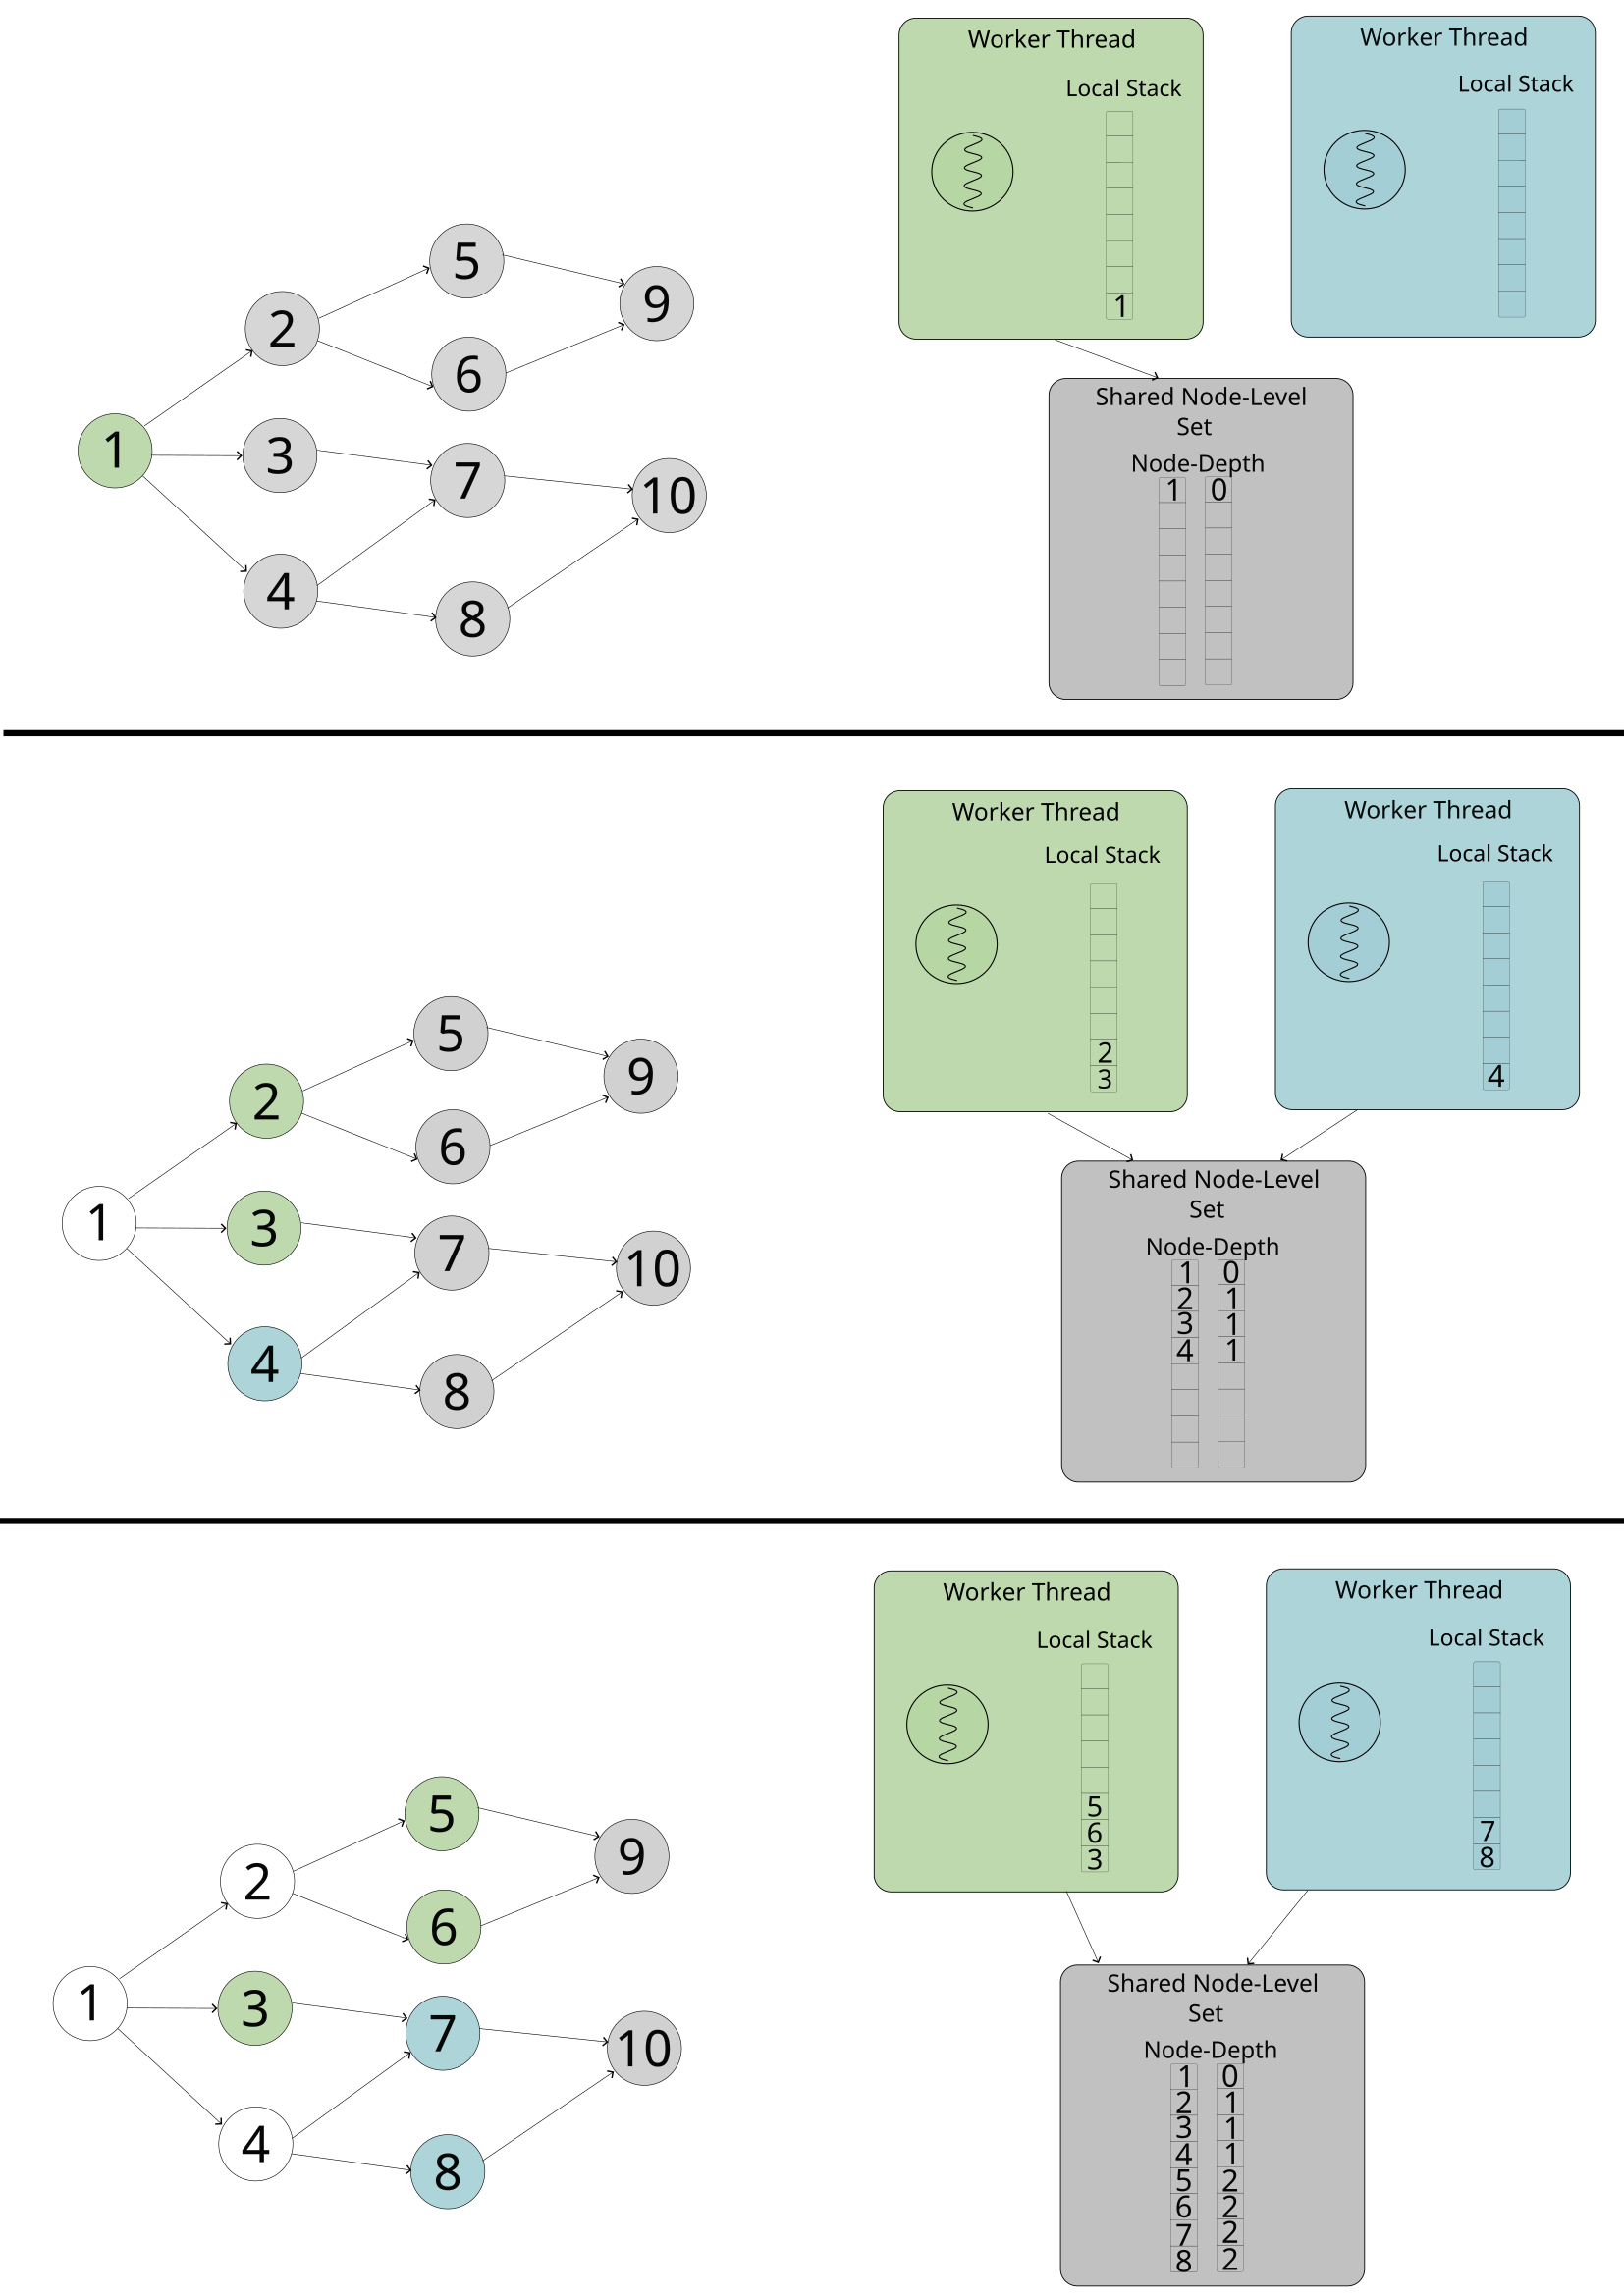
\includegraphics[width=0.75\textwidth]{figures/parallelDFS.png}
    \caption{Parallel DFS}
    \label{fig:parallelDFS}
\end{figure}
